%*----------- SLIDE -------------------------------------------------------------
\begin{frame}[t]{Finalização}
    \begin{itemize}
        \item Cada líder deverá realizar a apresentação final do desafio no dia 25/maio/2020.
        \item No dia da apresentação, somente o líder poderá responder os questionamentos emitidos pelos facilitadores.
        \item A avaliação será da equipe, não havendo avaliação individual dos integrantes da equipe com exceção do líder de cada equipe.
        \item A apresentação deverá ser desenvolvida em latex.
        \item Os videos dos desafios deverão estar contidos na apresentação final.
        \item Os videos deverão ser completos, tendo começo, meio e fim da missão realizada.
    \end{itemize}
%*----------- notes
    \note[item]{Notes can help you to remember important information. Turn on the notes option.}
\end{frame}
%-
%*----------- SLIDE -------------------------------------------------------------
\begin{frame}[c]{A importância atual da robótica}
    \begin{center}
        % \movie[loop,width=0.6\linewidth,height=0.3375\linewidth,showcontrols=false,autostart]{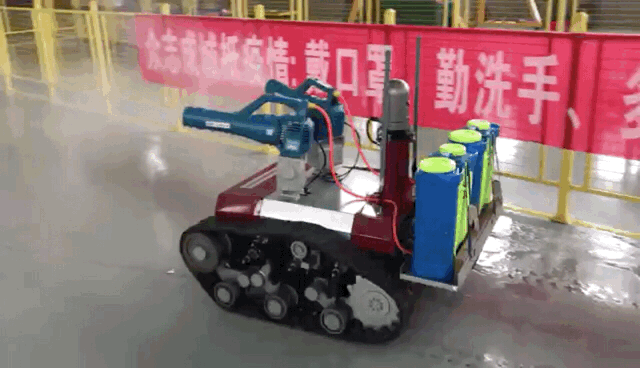
\includegraphics[width=0.6\textwidth]{Media/gifs/robotdesinfec0.png}}{Media/gifs/robotdesinfec.wmv}
    
        \includemedia[
            width=0.7\linewidth,
            totalheight=0.39375\linewidth,
            activate=pageopen,
            passcontext, 
            %transparent,
            addresource=./Media/gifs/robotdesinfec.wmv,
            flashvars={
            source=./Media/gifs/robotdesinfec.wmv
            &autoPlay=true
            &autoRewind=true
            &loop=true}
            ]{\fbox{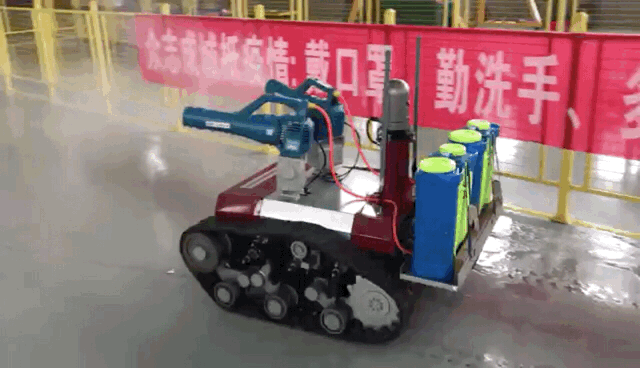
\includegraphics{Media/gifs/robotdesinfec0.png}}}{VPlayer.swf}
    \end{center}
%  %\movie[width=8cm,height=4.5cm]{test}{../Movies/Darwin-OP.mp4}

% % \includemedia[
% %     width=0.4\linewidth,
% %     totalheight=0.225\linewidth,
% %     activate=pageopen,
% %     passcontext,  %show VPlayer's right-click menu
% %     addresource=../Movies/Darwin-OP.mp4,
% %     flashvars={
% %       %important: same path as in `addresource'
% %       source=../Movies/Darwin-OP.mp4
% %     }
% %   ]{\fbox{Click!}}{VPlayer.swf}

%     \pdfpcmovie{\includegraphics[width=\textwidth]{Darwin-OP}}{Darwin-OP.mp4}

%*----------- notes
    \note[item]{Notes can help you to remember important information. Turn on the notes option.}
 \end{frame}
 %-